In this chapter, we present the results of applying our improved metadynamics method to study nucleation of a model monoatomic Lennard-Jones liquid argon.  First, we will present the system studied, followed by real-space and structural results of the simulation that provide evidence that nucleation is occurring.  Next, we perform analysis of the energy landscape to extract the energy barriers involved in the nucleation process.  Finally, we make estimates to the nucleation rates and extend the metadynamics method to time.  

\section{System}
In this study, we chose to apply the metadynamics method to a model liquid argon system, modeled by the Lennard-Jones potential.  Lennard-Jones potential is the most common potential applied in computer simulations due to its simplicity and accuracy in matching the pair potential of argon.  Due to the complexity of the nucleation process, we desired a simple potential such as the Lennard-Jones potential in order not to make the problem more complex than it already is.  Further, Lennard-Jones is an  well studied and understood potential, thus there is a vast amount of literature available for us to compare our results with \cite{HANSEN2006v}.  

\begin{figure}[h]
	\centering
	\includegraphics[width = .5\textwidth]{./Figures/Nucleation/LJ_potential.pdf}
	\caption[The Lennard-Jones potential is plotted as a function of atomic distance.  The potential is also separated into the repulsive and attractive contributions.  Key features of the potential such as the minimum energy and distance are shown.]{The Lennard-Jones potential is plotted as a function of atomic distance.  The potential is also separated into the repulsive and attractive contributions.  Key features of the potential such as the minimum energy and distance are shown. \cite{Jones463}}
	\label{LJ}
\end{figure}

Figure \ref{LJ} shows the pair potential for Lennard-Jones liquid.  A pair potential determines the potential energy between two atoms in a simulation, the gradient of this pair potential determines the force exerted by two atoms on one another.  The Lennard-Jones pair potential (also known as the 12-6 potential) is
\begin{equation}
U(r) = 4\epsilon\left[\left(\frac{\sigma}{r}\right)^{12} - \left(\frac{\sigma}{r}\right)^6\right]
\end{equation}
where $U$ is the potential, $r$ is the distance between two atoms centers, $\epsilon$ is the strength of the interaction between two atoms, and $\sigma$ is the ``radius'' of the atom \cite{Jones463}.  In this potential, as shown in Figure \ref{LJ}, the 12 term represents the repulsive force between atoms and the 6 term represents the attractive term between atoms.  The net force has a minimum at a distance $2^{1/6}\sigma$ resulting in an energy of $-\epsilon$.   The Lennard-Jones potential is well shown to crystallize to an FCC crystal, which as discussed previously, is easily distinguishable with $\bar{q}_6$.

For this thesis the Lennard-Jones parameters were chosen as the following, $\sigma$ of 3.40 \AA, $\epsilon$ of 0.9977 kJ/mol.  This results in a $r_o$, minimum energy distance, of 3.82 \AA.  This is important for determining the lattice constant of the crystal structure.  Each atom had a mass of 39 amu.  For these simulations, the cutoff distance for force calculations was 1.0 nm or 10 \AA.  These simulations had no electrostatic force calculation.  Neighbor searching was performed with grid search and a Verlet cut-off scheme \cite{Verlet1967}.  

For this thesis, we studied the nucleation process with two separate system densities, one high and one low.  The high density system was constructed such that the density of the system matched that of the crystalline state for Lennard-Jones argon.  Lennard-Jones argon has an FCC crystal structure and has a reported lattice constant of 5.24 \AA, which can be computed from knowledge of the FCC crystal structure and the minimum energy distance of the Lennard-Jones potential.  %maybe add calculation of this
The number of atoms was created such that in the crystal state, an unit cell is replicated six times in each direction.  Thus, the number of atoms is equal to 4$\times$6$^3$, or 864 atoms with a fixed box length of 3.0, this results in a density of ~1.25 in Lennard Jones units.  The system was generated with a random configuration of atoms, and then, underwent energy minimization.  An NVT simulation was then performed to equilibrate the system.  The NVT simulation was 100 ps with a 1 fs time step at a fixed temperature of 120 K, well above the freezing temperature.

The high density system was produced to reflect the density of a perfect FCC crystal of the final state of the simulation.  To compare, we also ran a simulation at a lower density that reflects the density of the liquid state.  This system was equilibrated with an NPT simulation with ambient pressure to equilibrate the box length, and therefore the density of the system.  The NPT simulation was for 200 ps, at a temperature of 1 in Lennard-Jones units (120 K).  This system had a density of 0.728 in Lennard-Jones units.  Following the NPT simulation an NVT simulation was performed for 100 ps at a temperature of 1 in Lennard-Jones units (120 K).

The previous paragraphs described the preparation protocols for the two system densities studied.  These two systems were then used as the starting point for the metadynamics simulations.  As proof that the two simulations began from an amorphous metastable state, we calculated the pair distribution function for each system, shown in Figure \ref{gofr} \cite{HANSEN2006v}.  The figure shows that both systems are in an amorphous state.  The high density system has a higher first peak due to the increased density of the system, but the lack of strict peaks in the pair distribution function allows us to assume the system is not ordered. 

\begin{figure}[h]
	\centering
	\includegraphics[width = .45\textwidth]{./Figures/Nucleation/high_density/g_r.pdf}
	\hspace{.03\textwidth}
	\includegraphics[width = .45\textwidth]{./Figures/Nucleation/low_density/g_r.pdf}
	\caption{Pair distribution function of the equilibrated system configurations.  Figure A shows the pair distribution function for the high density system, and Figure B shows the pair distribution function for the low density system.}
	\label{gofr}
\end{figure}  

Next, we performed metadynamics simulations on the two different density systems.  Both metadynamics simulations were carried out with the following parameters.  The energy convergence criteria was set to 10e$-$8 for the smallest change in system energy, the starting minimization parameter was 10e$-$4 nm (this was shown in the previous chapter to be sufficiently small), the maximum number of energy minimization steps was set to 7000, the penalty function height was set to 1 kJ/mol (also 1.00 in Lennard-Jones units), the penalty function width squared was .1 nm$^2$ (or 0.865 in Lennard Jones units), and the maximum number of penalties applied was 20,000 (however the simulations usually exceeded wall-time allocation prior to this criteria).  As for the GROMACS run parameters for pair potential calculations, the cut-off for force calculations was 1 nm, and periodic boundary conditions were used.  

\section{Real Space and Structure}
In this section, we will present the results of the metadynamics simulations of the two different density systems.  The metadynamics method we implemented into GROMACS results in several outputs, the potential energy at every minimization step, the added potential at every minimization step, the step size at every minimization step, the potential energy at the convergence of energy minimization, the number of steps to obtain convergence, the real space trajectory of the simulation as a function of minimization step, and the $\bar{q}_6$ value for every atom at convergence of energy minimization.  The bond order parameter was also calculated by LiquidLib (discussed in Appendix \ref{LiquidLib}), a post processing package for analyzing atomic scale trajectories created by our research group, after the simulation for the trajectory as a function of minimization step.  The bond order parameter was needed at every step for later processing, and metadynamics only provides this at the end of energy minimization.  For the two system densities studied the potential energy sampled by the metadynamics simulations are shown in Figure \ref{landscapes}.

\begin{figure}[h]
	\centering
	\includegraphics[width = .45\textwidth]{./Figures/Nucleation/high_density/landscape.pdf}
	\hspace{.03\textwidth}
	\includegraphics[width = .45\textwidth]{./Figures/Nucleation/low_density/landscape.pdf}
	\caption{Potential energy in kJ/mol versus penalty number.  These figures represent the energy landscape sampled by the metadynamics simulation.  The blue line is the energy landscape, the green circles are energy barriers or saddle points, and the red squares are energy minimums or basins.  The figure on the left is for the high density simulation, and the figure on the right is for the low density simulation.  The letters in the left figure correspond to the panels in Figure \ref{simulation}.}
	\label{landscapes}
\end{figure}

Figure \ref{landscapes} shows the sampled energy landscapes for the two different density systems studied.  The figures show many rich features.  First, the landscapes were processed to find which penalty functions resulted in the sampling of an energy barrier (saddle point) or a new energy minimum (basin), which are represented in green circles and red squares respectively.  At first glance, the potential energy of the high density system is considerably lower than that of the low density case.  This is expected since the high density case is under pressure, thus the atoms are pushed closer to the equilibrium distance.  In the low density system, the added free space results in the atoms being further spaced from one another.  Thus, from Figure \ref{LJ}, we can see that if atoms are closer to $r_o$ the pair potential is less than when spaced greater than $r_o$.  In the low density case, the atoms are not compressed near one another, so the energy is further from the minimum pair potential, we could also conclude this from looking at the pair distribution plots shown previously.  Second, the low density case has significantly more penalties applied than the high density case.  This is just a result of computational complexity.  Depending on the speed with which energy minimization converges directly determines the number of penalties that can be applied.  However, this may also result from the landscape being simpler (smoother) for the low density case.

The most important feature to notice in the two figures is the clear plateaus at certain energies.  These represent large basins in the energy landscape.  These two figures show an important feature of the energy landscape, the density dependence of the landscape.  The two figures show that as the density is increased the landscape is roughened and more complex.  The high density case has many more saddle points, whereas the low density case appears to have shorter neighboring saddle points.  The low density landscape seems smoother, and there are clear jumps from one large basin to another.  Further, there is an initial immediate decrease in potential energy for the low density system, after only a few penalties.  Whereas, the high density system requires many penalties before its first major transition.  The high density case has many basins between the large basins that the system gets caught in along the way.  In fact, there is a theory that if the density is decreased sufficiently, the landscape simplifies to the point that only one basin exists (the perfect crystalline state).  We believe this lends support to this density dependence theory of the landscape.

\begin{figure}[h]
	\centering
	\includegraphics[width = .45\textwidth]{./Figures/Nucleation/mtd_amorphous.png}
	\hspace{.03\textwidth}
	\includegraphics[width = .45\textwidth]{./Figures/Nucleation/mtd_prenucleation.png}
	\vspace{5mm}
	\\
	\includegraphics[width = .45\textwidth]{./Figures/Nucleation/mtd_nucleation.png}
	\hspace{.03\textwidth}
	\includegraphics[width = .45\textwidth]{./Figures/Nucleation/mtd_crystal.png}
	\caption{Real space visualization of one of the simulations.  The atoms are colored by the $\bar{q}_6$ value, blue representing a low value (disordered state) and red representing a high value (ordered state).  The figures are ordered such that going from A to D the number of penalties applied to the system increases.  The figures also correspond to the same letter in Figure \ref{landscapes} A, thus showing the difference in system energy at the different points in the simulation as a function of structure.}
	\label{simulation}
\end{figure}

While much can be learned from just looking at the energy landscape itself, the landscape is even more insightful when viewed simultaneously with a real space representation of the simulation.  Figure \ref{simulation} shows the real space representation of the simulation.  The letters in the sub figures correspond with the letters in Figure \ref{landscapes}.  This is to show the clear structural change in the system after a large basin transition occurs.  The figures are colored based on the bond order parameter, blue meaning amorphous and red meaning ordered.  Panel A shows the system in an amorphous state, or a high energy state on the landscape.  As penalties are applied the system overcomes many small local saddle points, which results in small local rearrangements of the atoms.  By point B, the system has undergone many small rearrangements leading to a small decrease in energy and select few pre-critical atoms forming.  These pre-critical atoms have small amounts of order and are grouped together.  At this point, as more penalties are applied the system transitions from one metastable basin to another, from B to C, and a large scale rearrangement of atoms occurs.  At point (panel) C the system energy has dropped significantly and the nucleation sites have formed, generally near where the critical atoms were in point (panel) B.  Point (panel) C shows that areas of high order now exist and a crystalline phase can be seen in these regions.  As more penalties are applied, small rearrangements occur again as the system samples the new metastable basin.  Then after several penalties are applied the system under goes a large transition again, and becomes a near perfect crystal shown in point (panel) D.  This point has the lowest potential energy and has near uniform high bond order parameters.

By watching the real space representation, and the energy landscape, we can see the crucial events involved in the phase change process.  We did not show the real space representation for both densities because they show similar events and would thus be extraneous to show both.  Another important way to view the simulation is from the perspective of the structure in the system.  Figure \ref{structure} shows the structure in the system as a function penalty function applied.

\begin{figure}[h]
	\centering
	\includegraphics[width=.45\textwidth]{./Figures/Nucleation/high_density/heatplot_bar.png}
	\hspace{.03\textwidth}
	\includegraphics[width=.45\textwidth]{./Figures/Nucleation/high_density/Q6_landscape.pdf}
	\caption{Structural evolution of the simulation shown in Figure \ref{simulation}.  The left figure shows the distribution of $\bar{q}_6$ values as a function of penalty applied to the system.  The color bar is the probability of a given $\bar{q}_6$ value.  The right figure shows the system wide bond order parameter $Q_6$ and the potential energy of the system versus penalty applied to the system.  The blue line is the system wide bond order parameter and the orange line is the energy landscape.}
	\label{structure}
\end{figure}

Figure \ref{structure} shows the distribution of bond order parameter values as a function of penalty number and shows the system wide bond order parameter as a function of penalty number.  The distribution of the bond order parameter values shows that the system starts with ubiquitously low $\bar{q}_6$ values.  The variance of these values is large.  This indicates the system is fully amorphous.  Then after the first large transition in the system the $\bar{q}_6$ distribution increases to a mean value just below the FCC value.  The variance is still large enough that we can see a portion of the distribution has exceeded the criteria for FCC ordered.  Then after the second transition, the distribution surpasses the FCC criteria value and the distribution becomes discrete in value.  Similarly, we noticed that if we plotted the system wide bond order parameter, $Q_6$, alongside the energy landscape, the two values followed a very similar trend.  This just further confirms that more ordered has lower system potential energy.

\section{Energy Barriers}
Computation of the potential energy landscape provides a great deal of information about a system.  The energy basins (energy minimums) provides structural information about the system as shown in the previous section.  Even more useful is the landscape saddle points (energy barriers) provides information about dynamical and kinetic events in the system.  By extracting the energy barriers from the energy landscape, the evolution of the system can be better understood.  In order to understand the nucleation and crystal growth process, the energy barriers from the landscape can elucidate the process, however, these two events have distinct energy barriers, thus a method to extract two energy barriers from the landscape is needed.

\begin{figure}[h]
	\centering
	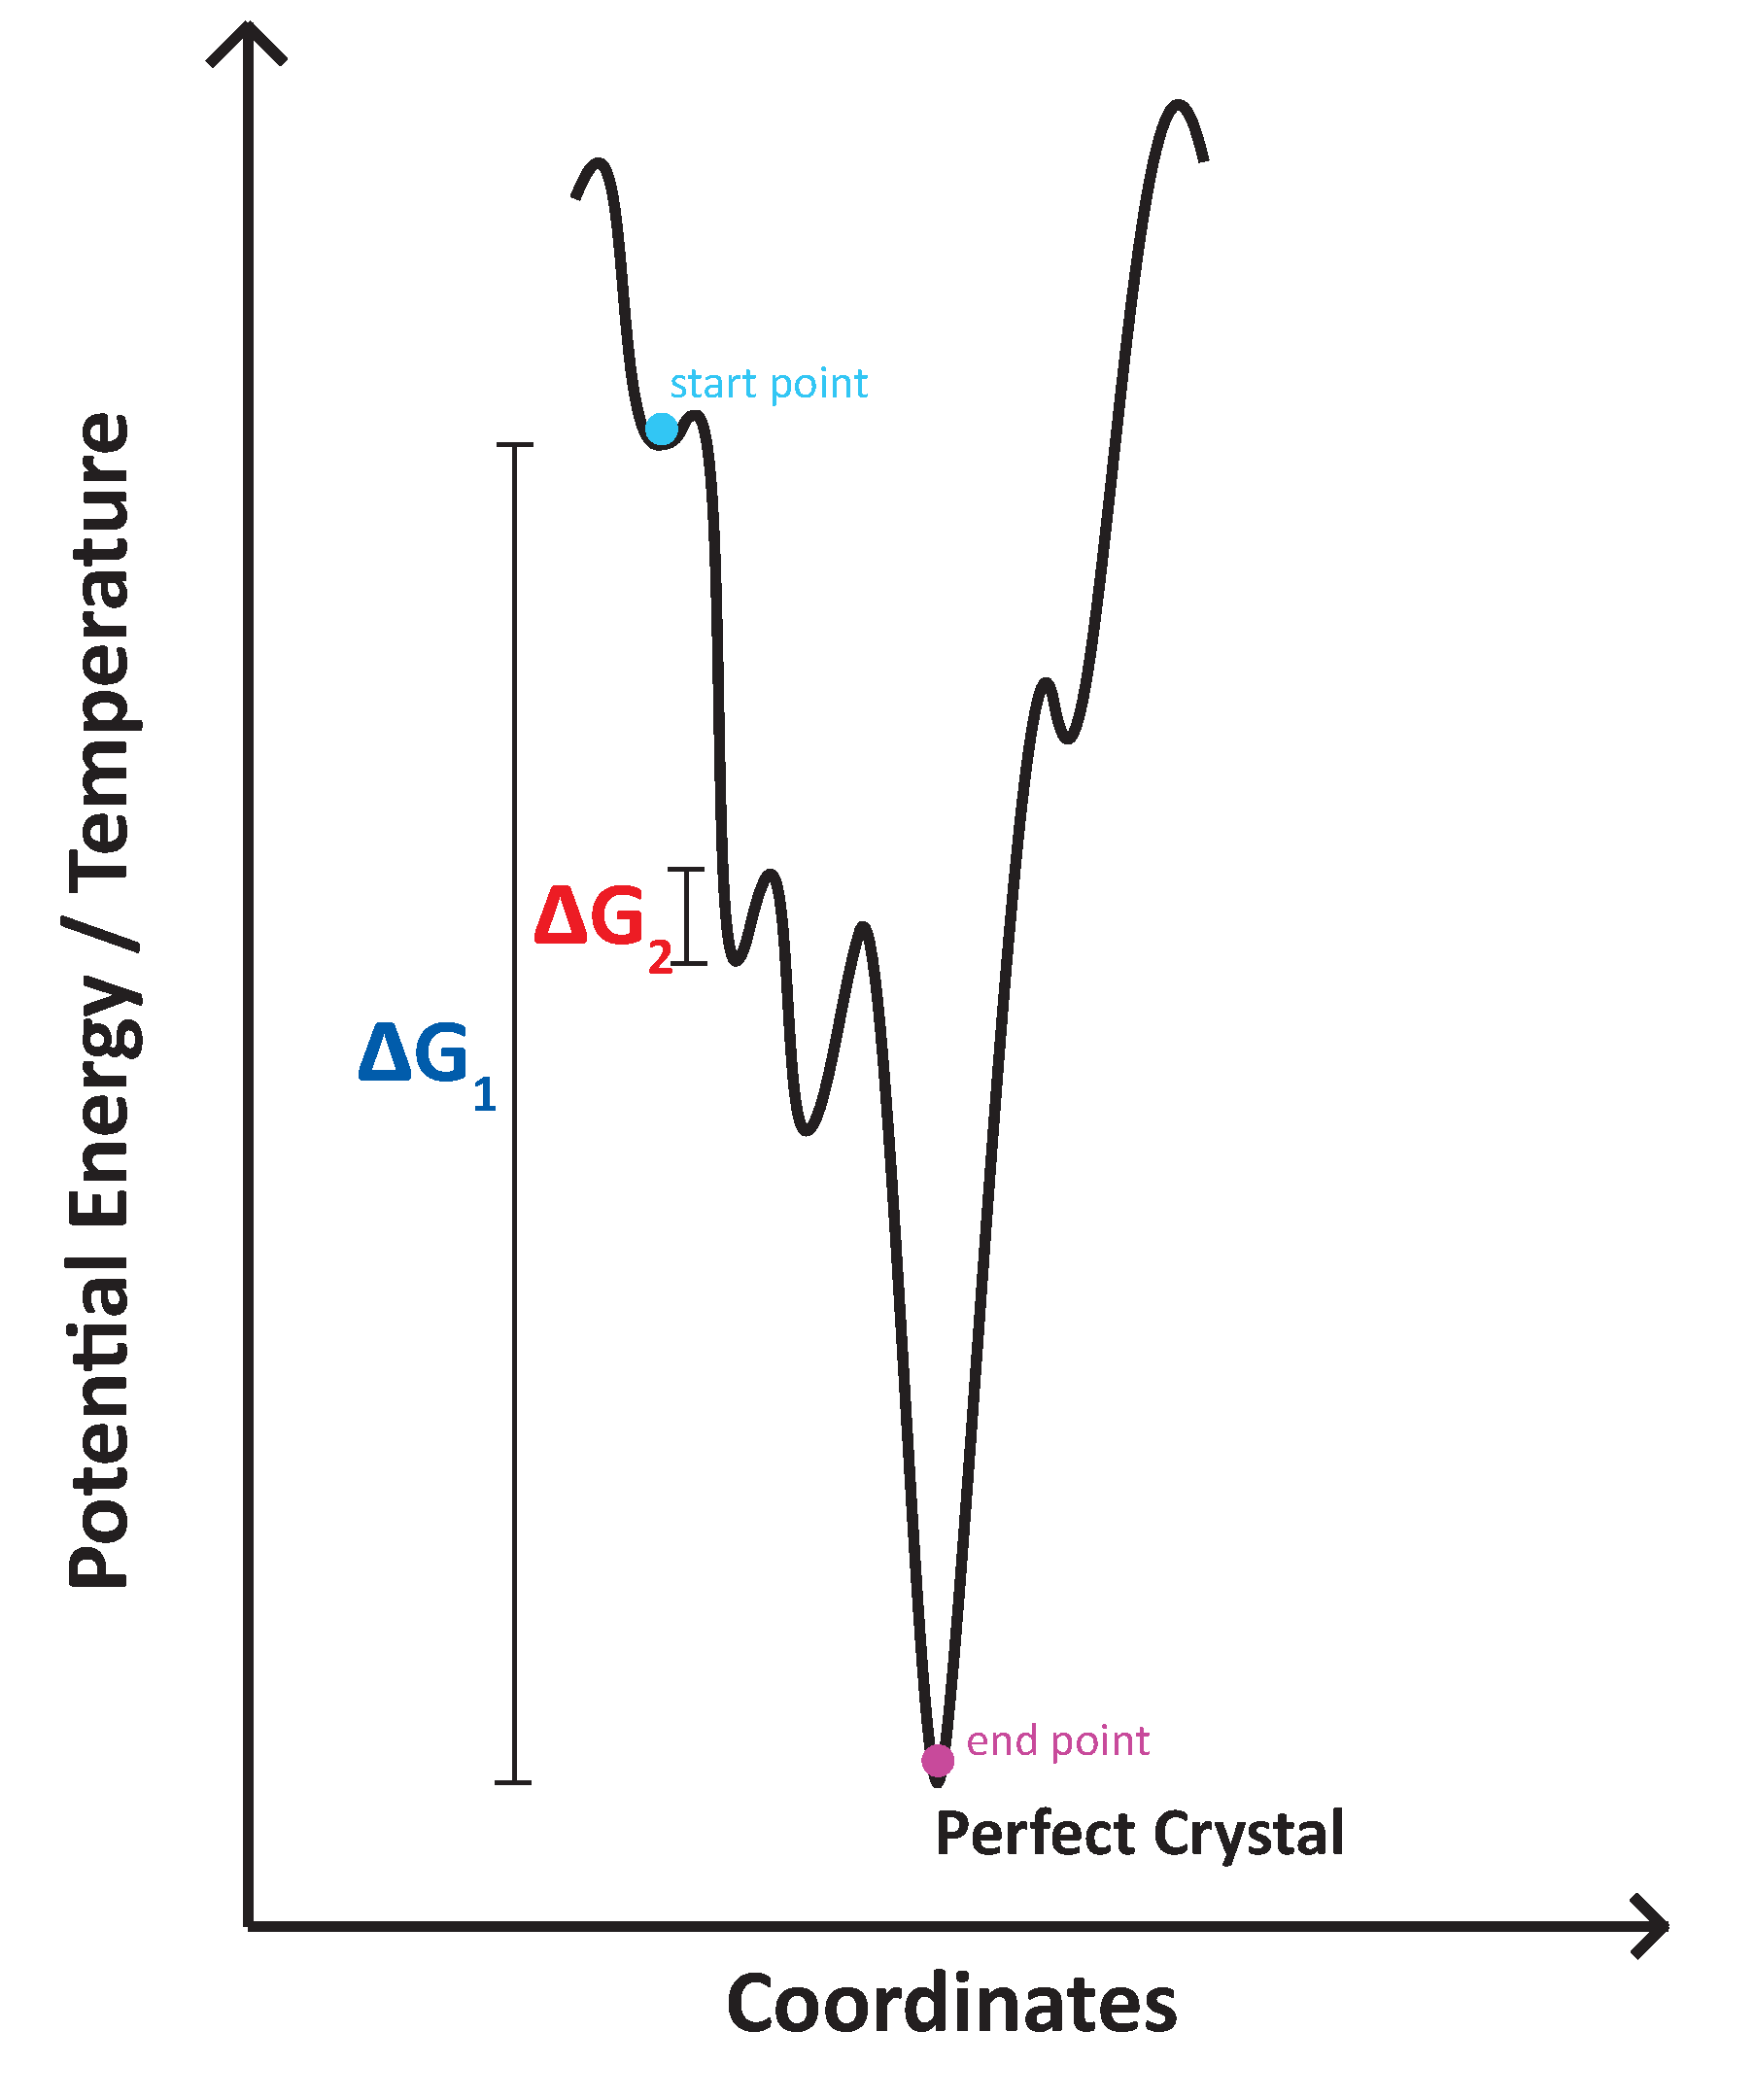
\includegraphics[width=.5\textwidth]{./Figures/Nucleation/nucleation_landscape.pdf}
	\caption{This figure shows a schematic drawing of the energy differences calculated from the energy landscape.  The colors for $\Delta G$ 1 and 2 correspond to the colors in Figure \ref{barriers}.  $\Delta G_1$ is the energy difference between the perfect crystal state and a given energy landscape basin.  $\Delta G_2$ is the energy difference of between the neighboring saddle point and the energy basin.  The schematic drawing also shows the starting point and end point of a theoretical metadynamics simulation along the energy landscape.}
	\label{barriers_origin}
\end{figure}

Figure \ref{barriers_origin} shows how the energy barrier for nucleation and crystal growth can be extracted from the energy landscape.  The schematic drawing that the starting point is from a high energy basin, and the end point is the perfect crystal lowest energy basin.  Between the two basins is a series of energy barriers and energy basins that are sampled along the way.  The figure shows the two energy differences involved in the simulation.  The first energy difference is the neighboring energy barrier separating two energy basins.  As explained previously, this is the energy barrier for dynamical behavior.  In this study, we assume that this barrier is the barrier for crystal growth.  This is justified by the idea that as an energy barrier is crossed the subsequent basin is of lower energy and generally greater structure.  Therefore, this barrier is the barrier for the addition of atoms to the new phase.  Similarly, since these barriers generally represent dynamics, such as atomic diffusion, and crystal growth is generally believed to be dictated by the diffusion of atoms to the crystal site, we logically connected these energy barriers to the crystal growth process.  This barrier is colored red to correspond to the color in the subsequent figures.  

The second energy difference in the system is the difference in system energy between the energy basins and the lowest energy basin energy.  This energy difference labeled $\Delta G_1$, is the difference between the perfect crystal state and the two phase (liquid and solid) or the single phase (liquid) state.  We have equated this energy difference to the energy required for formation.  This connection comes from the idea that to introduce the new phase comes with a certain energy cost, and this energy difference is the cost of the new phase induction.  This is similar to the CNT idea of calculating the nucleation free energy barrier.  However, rather than calculate the energy difference as a function of cluster radius as CNT does, we have calculated this energy difference without any macroscopic properties or \textit{a priori} assumptions about cluster shape.  This energy difference is also colored to correspond to subsequent figures.

\begin{figure}[h]
	\centering
	\includegraphics[width = .45\textwidth]{./Figures/Nucleation/high_density/TemperatureMapping.pdf}
	\hspace{.03\textwidth}
	\includegraphics[width = .45\textwidth]{./Figures/Nucleation/low_density/TemperatureMapping.pdf}
	\caption{Temperature mapping for the two simulations.  The left figure is for the high density system and the left figure is for the low density system. Red open circles are the data points from MD simulations, and the blue line is the data fit from the equation listed in the figure.}
	\label{temperature}
\end{figure}

As discussed in the previous chapter, in order to obtain useful information from the energy landscape is to be able to project the analysis into temperature.  Figure \ref{temperature} shows the two temperature mappings for the two system densities.  Before applying these to the energy landscape, the two figures show very distinct features.  First, the range over which the transition of high energy to low energy states occurs is dramatically different for the two systems.  The low density system has a transition over roughly ~30 K and the high density occurs over roughly ~10 K.  Further, for the high density case, there is a larger variance in values below the transition temperature than in the low density case.  Presumably this is due to the rougher energy landscape of the high density case, which means that it is easier for the system to be trapped in a metastable state than in the low density  case.  It is important to note that the data fit for the high density case is biased to pass through the lowest energy state rather than through points that reduce the residual, because if the fit does not cover the full range of energy values of the energy landscape then the mapping of the landscape to temperature fails.  The transition temperature for each density will be discussed later.

\begin{figure}[h]
	\centering
	\includegraphics[width = .45\textwidth]{./Figures/Nucleation/high_density/activation_energies.pdf}
	\hspace{.03\textwidth}
	\includegraphics[width = .45\textwidth]{./Figures/Nucleation/low_density/activation_energies.pdf}
	\caption{The activation barriers calculated from each simulation versus temperature.  The left figure is for the high density system and the right figure is for the low density system.  The figures show the activation barrier for crystal growth in red circles, the formation of a nucleation site in blue squares, and the total (sum of the two) in green triangles.  }
	\label{barriers}
\end{figure}

Extracting the energy differences from the sampled energy landscape and mapping to temperature are shown in Figure \ref{barriers}.  Figure \ref{barriers} shows the formation energy in blue squares, the growth energy in red circles and the total in green triangles.  There are many important features displayed in these figures.  First the two figures show a clear non-monotonic nature to the total energy difference in the system.  Second, the figure shows that different energies dominate at different temperature regimes.  At low sub cooling, the formation energy is high and thus nucleation sites are rarely formed.  At high sub cooling the formation energy is low and thus nucleation can occur more readily.  On the other hand, at low sub cooling the growth energy is low, because dynamics are quicker in this regime.  At high sub cooling the growth energy is high, because the dynamics are much slower as the glass transition temperature is reached.  Clearly from this figure, the low subcooling regime is dominated by formation energy differences, and at high subcoolings the regime is dominated by growth energy differences.  The high density figure did not show increase in total energy at lower temperatures most likely from lack of sampling a lower temperature regime, we believe if the data set was extended to lower temperatures the total energy would turn upwards again like in the low density case.

\section{Nucleation Rate and Interpolation to Time}
At this point, we employ classical nucleation theory.  While classical nucleation theory has been shown to inaccurately predict the free energy barrier involved in nucleation and crystal growth, the use of free energy differences to calculate the rates is still considered a correct methodology.  Classical nucleation makes the claim that the nucleation rate is proportional to the energy barrier by the following equation
\begin{equation}
\dot{N} \propto \exp\left( -\frac{\Delta G_{formation}}{k_BT}\right)
\end{equation}
where $\dot{N}$ is the nucleation rate.  We believe that with the metadynamics method employed in this study we have more accurately calculated the free energy barrier needed to calculate the nucleation rate.  Similarly, the crystal growth rate is calculated by
\begin{equation}
\dot{I} \propto \exp\left( -\frac{\Delta G_{growth}}{k_BT}\right)
\end{equation}
By using these equations, the trend of the nucleation, crystal growth, and overall crystallization rate is plotted in Figure \ref{rates}.  The overall rate is equal to the product of the nucleation rate and the crystal growth rate.

\begin{figure}[h]
	\centering
	\includegraphics[width = .45\textwidth]{./Figures/Nucleation/high_density/trend.pdf}
	\hspace{.03\textwidth}
	\includegraphics[width = .45\textwidth]{./Figures/Nucleation/low_density/trend.pdf}
	\caption{Exponential of the activation barriers versus temperature.  The left figure is for the high density system, and the right figure is for the low density system.  The red circles is for the growth of a nucleation site, the blue squares are for the formation of a nucleations site, and the green triangles are the sum of the two.  The pre-factor $J_o$ is the factor to relate these quantities to the crystallization rate of the system.  }
	\label{rates}
\end{figure}

Figure \ref{rates} shows the temperature dependence of the nucleation, crystal growth, and crystallization rate as determined by the energy barriers calculated from the metadynamics simulations.  From these figures, we can see that at low sub cooling the phase transition is limited by the formation rate and the growth rate is high.  Similarly, at high sub cooling the transition is limited by the growth rate due to slow dynamics of the system.  Further, we see that at a particular temperature roughly 301 K and 45 K for the high density and low density systems respectively, the overall rate has a maximum, and there is a transition from growth dominated to formation dominated.  As discussed in the introduction, this is expected.  

\begin{figure}[h]
	\centering
	\includegraphics[width=.45\textwidth]{./Figures/Nucleation/LJ_phase_density.png}
%	\hspace{.03\textwidth}
%	\includegraphics[width=.45\textwidth]{./Figures/Nucleation/Lj_transition_temperature.png}
	\caption[Coexistence curve for Lennard-Jones argon system as a function of normalized density and normalized temperature in Lennard-Jones units. F represents the fluid regime, G is for gaseous and L is for liquid, and S is for solid or crystalline.  The dashed horizontal line at around T = .7 Lennard Jones units is the coexistence line for freezing from a liquid to a solid.  This is also 84 K.]{Coexistence curve for Lennard-Jones argon system as a function of normalized density and normalized temperature in Lennard-Jones units \cite{Hansen1969}. F represents the fluid regime, G is for gaseous and L is for liquid, and S is for solid or crystalline.  The dashed horizontal line at around T = .7 Lennard Jones units is the coexistence line for freezing from a liquid to a solid.  This is also 84 K. \cite{Hansen1969}}
	\label{LJ_phase_density}
\end{figure}

As a sanity check that these temperatures in Figure \ref{rates} are physical, we can compare the results with a coexistence curve for Lennard-Jones shown in Figure \ref{LJ_phase_density} \cite{Hansen1969}.  Figure \ref{LJ_phase_density} shows the density versus temperature phase diagram \cite{Hansen1969}.  From this figure, we can see that for the low density case, of about 0.728 in reduced units, has a freezing temperature of 0.7 in reduced units, or 84 K.  This means that we are predicted that for homogeneous nucleation to occur, the system must be around 10 K sub cooled.  Further, at 40 K sub cooled, we see a maximum in transition rate.  The reported glass transition temperature for this density is roughly around ~24 K, thus for us to predict the rates to decrease near 30 K is reasonable.  Similarly, from Figure \ref{LJ_phase_density}, we can approximate the melting temperature for the high density system, of a about 1.25 in reduced units, to be near 360 K by extrapolation of the data in Figure \ref{LJ_phase_density}.  Further, we predict from our temperature mapping that a transition to landscape dominated to be near 310 K, or 50 K subcooling.  

One of the largest advantages to metadynamics, compared to Monte Carlo, is that the simulation can provide temporal information, which is generally macroscopically long compared to molecular dynamics.  It provides information about dynamics through the energy barriers.  However the simulation itself typically can not be analyzed as a function of time, because the simulation is a function of penalty number.  However, from the original energy landscape framework, the dynamical behavior is described as the transition from one basin to another.  Thus, from the metadynamics simulation, we consider that the simulation is a series of basin hopping.  Thus, if we know the average time for the transition from one basin to another, we can interpolate the metadynamics simulation to time \cite{Cavagna2009}.  We can predict this average time as the relaxation time for the system to relax from one basin to another.  The relaxation time for basin transitions is commonly displayed as
\begin{equation}
\tau = \tau_M\exp\left( \frac{E_A}{k_BT}\right)
\end{equation}
where $\tau$ is the relaxation time, $\tau_M$ is the Maxwellian relaxation time, $E_A$ is the activation energy for the transition \cite{Dexter2009}.  Thus, since we know the activation energy separating the energy basins sampled in the simulation, and the Maxwellian relaxation time can be calculated from an Arrhenius law
\begin{equation}
	\tau_M = \frac{\eta}{G_\infty}
\end{equation}
where $\eta$ is the viscosity and $G_\infty$ is the shear modulus \cite{Dexter2009}. The Maxwellian relaxation time is reported on the order of hundreds of femtoseconds \cite{Dexter2009}.  There is variability for the density, but for now, order is sufficient \cite{Dexter2009}.  By assuming the time to cross an energy barrier and transition from one basin to another, the energy landscape can be plotted as a function of time.

\begin{figure}[h]
	\centering
	\includegraphics[width=.45\textwidth]{./Figures/Nucleation/high_density/time.pdf}
	\caption{The energy landscape extrapolated from a function of penalty number to a function of time.}
	\label{time}
\end{figure}

Figure \ref{time} shows the energy landscape for the high density simulation as a function of time in picoseconds.  As a sanity check that this is the correct approach for time extrapolation, a research group used MD simulations of Lennard Jones argon with identical box size and number of atoms as we used \cite{Park2004}.  The group, knowing MD cannot capture nucleation, induced the nucleation process with a field \cite{Park2004}.  By inducing the nucleation event they studied the system over time \cite{Park2004}.  They used a time step of 5 fs and determined the system took 80,000 time steps to achieve a crystal state \cite{Park2004}.  The group also studied the energy landscape during the simulation and noticed a similar pattern of plateaus in the potential energy representing different structures in the system \cite{Park2004}.  By comparing this groups reported 400 ps time for crystallization, and Figure \ref{time} which shows we approximate a time of around 310 ps, we conclude that using the Maxwellian relaxation time and Arrhenius trend to extend our simulation into time is well founded.  We believe these two times are in good agreement given the relative error in relaxation time used, the MD simulation, and our own simulation.
